% !TEX root = ../main.tex
\begin{figure}[htbp]
\centering
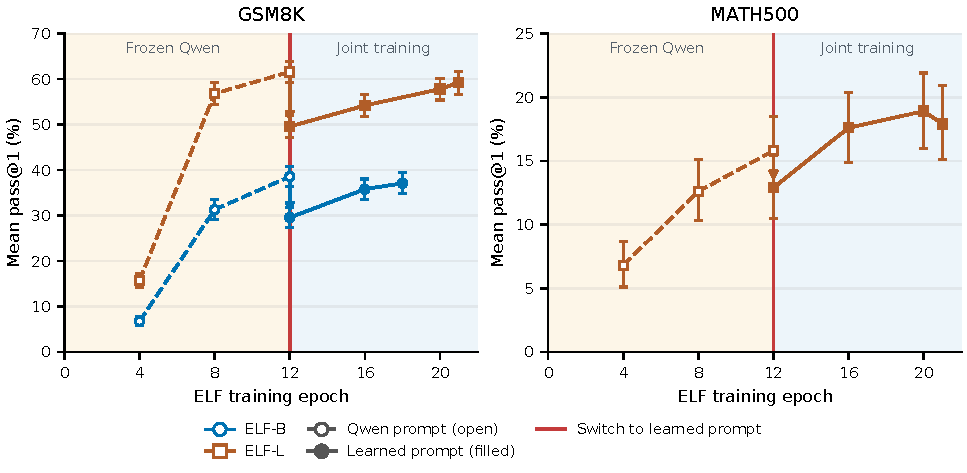
\includegraphics[width=\linewidth]{figures/prompt_curriculum_training.pdf}
\caption{\textbf{Stable teacher conditioning followed by learned prompt adaptation.} Pre-NFT learning curves, with GSM8K ELF-B/L together on the left and MATH500 ELF-L on the right. Open circles use Qwen prompt encoding; filled squares use the learned encoder. The vertical bar marks the epoch-12 substitution and start of joint training; arrows show the immediate MSE-prompt swap loss. Standalone prompt-MSE training leaves the ELF epoch fixed. Both axes start at zero; the first evaluated checkpoint is epoch 4. Points average seeds 42/123 at async $(2.5,2,1.5)$, 32 steps, and SCCFG 2; bars are 95\% problem-bootstrap intervals. ELF EMA is $0.9999$; prompt EMA is $0.999$ at the swap and $0.9999$ afterward.}
\label{fig:promptcurriculum}
\end{figure}
